
On March 11, 2011 a magnitude 9.1 earthquake struck Japan, the epicenter just 76km from the eastern coast of the Tohoku region.  This caused a tsunami that collapsed a nearby nuclear reactor resulting in the Fukushima Daiichi Nuclear Disaster, a meltdown that resulted in 19,500 total deaths.  The reactor was built to withstand earthquakes up to 8.6 in magnitude.

The following example, inspired by (Silver, 2015)\cite{silver2015signal} illustrates a statistical model of annual earthquake frequencies of the greater Tohoku region.
Data was queried using the United States Geological Survey's ANSS Comprehensive Earthquake Catalog (ComCat).  The full analysis was conducted in R and is detailed in the appendix of this thesis.
After pre-processing, the data was coerced into a table of magnitudes rounded to one decimal place and the following plot generated to display the annual frequency of magnitudes \textit{at or above} each size earthquake.

\begin{figure}[H]
    \center
    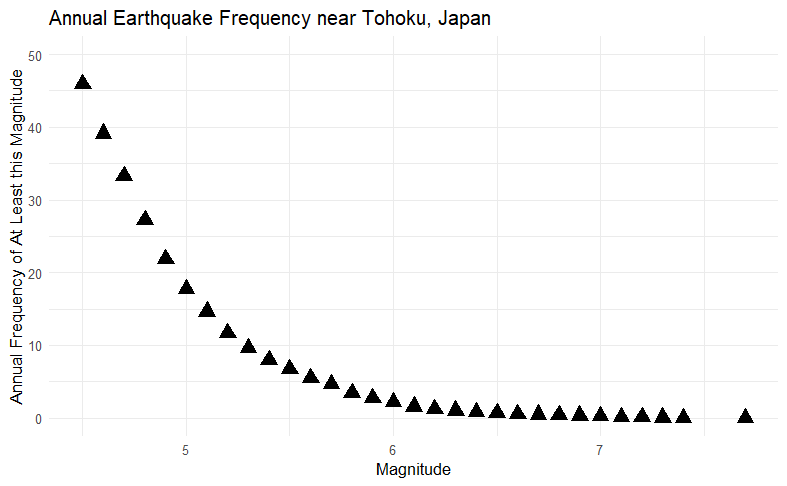
\includegraphics[width=0.75\linewidth]{Figures/tohoku_standardscale.png}
   % \vspace{-10pt}
    \caption{\footnotesize{Annual Tohoku earthquake frequencies of magnitude 4.5 and above.}}
    \label{tohoku_unfit}
\end{figure}

\subsubsection{Poisson Regression Models}
To establish a baseline to compare against neural networks, a Poisson regression model is fit. Data was split 80/20 for training and testing respectively.  

\begin{verbatim}
## 
## Call:
## glm(formula = freqc ~ mag, family = "poisson", data = train)
## 
## Deviance Residuals: 
##      Min        1Q    Median        3Q       Max  
## -0.39403  -0.20754  -0.02925   0.08617   0.22166  
## 
## Coefficients:
##             Estimate Std. Error z value Pr(>|z|)    
## (Intercept)  13.0940     0.7242   18.08   <2e-16 ***
## mag          -2.0467     0.1474  -13.88   <2e-16 ***
## ---
## Signif. codes:  0 '***' 0.001 '**' 0.01 '*' 0.05 '.' 0.1 ' ' 1
## 
## (Dispersion parameter for poisson family taken to be 1)
## 
##     Null deviance: 373.0667  on 23  degrees of freedom
## Residual deviance:   0.7758  on 22  degrees of freedom
## AIC: Inf
## 
## Number of Fisher Scoring iterations: 3
\end{verbatim}

This shows that for every unit increase in magnitude, the expected difference in the logs of annual frequency is -2.0467.  The test error for this model, as will be for future models, was calculated by the mean squared error between predicted test values and actual test values.  This turned out to be 0.03940496.  A plot of the data with the regression line is shown below:


\begin{figure}[H]
    \center
    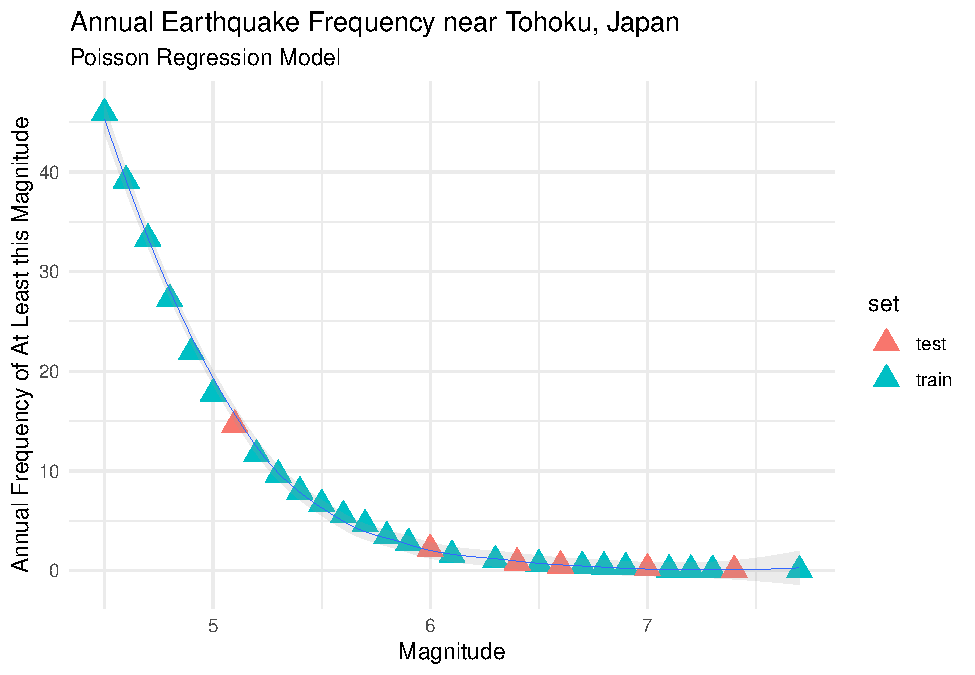
\includegraphics[width=0.75\linewidth]{Appendix_eq_files/figure-latex/unnamed-chunk-3-1.pdf}
   % \vspace{-10pt}
    \caption{\footnotesize{A Poisson regression line fit to the data.}}
    \label{tohoku_unfit}
\end{figure}

\begin{comment}

% latex table generated in R 4.2.2 by xtable 1.8-4 package
% Wed May  3 23:37:00 2023
\begin{table}[ht]
\centering
\begin{tabular}{rlr}
  \hline
 & Model & Test Error \\ 
  \hline
 & Poisson Regression &  0.03940496\\ 
   \hline
\end{tabular}
\end{table}

\end{comment}